\section{环境相机}\label{sec:环境相机}
光线追踪相比扫描线或基于栅格化的渲染方法的一个优点是
它容易利用特殊的图像投影。
在图像样本位置如何映射到光线方向方面我们有很大自由,
因为渲染算法不依赖诸如场景中的直线总是投影为图像中的直线那样的性质。

本节中,我们将介绍绕场景中一点追踪所有方向光线的相机模型,
它给出自该点可见的一切内容的2D视图。
考虑场景中绕相机位置的球;选择该球上的点给定追踪光线的方向。
如果我们用球坐标将该球参数化,则球上的每个点与一对$(\theta,\phi)$关联,
其中$\theta\in[0,\pi]$且$\phi\in[0,2\pi]$
(见\refsub{球坐标上的积分}关于球坐标的更多细节)。
这类图像尤其有用,因为它表示场景中一点的所有入射光
(这类图像表示的一个重要用处是环境光照——场景中使用光的基于图像的表示的渲染技术)。
\reffig{6.14}展示了San Miguel模型中的该相机。
$\theta$值范围从图像顶端的0变到图像底端的$\pi$,
$\phi$值范围由图像左侧到右侧从0变到$2\pi$
\footnote{熟悉制图学的读者会认出这是个\keyindex{等距柱状投影}{equirectangular projection}{projection投影}。}。
\begin{lstlisting}
`\initcode{EnvironmentCamera Declarations}{=}`
class `\initvar{EnvironmentCamera}{}` : public `\refvar{Camera}{}` {
public:
    `\refcode{EnvironmentCamera Public Methods}{}`
};
\end{lstlisting}
\begin{figure}[htbp]
    \centering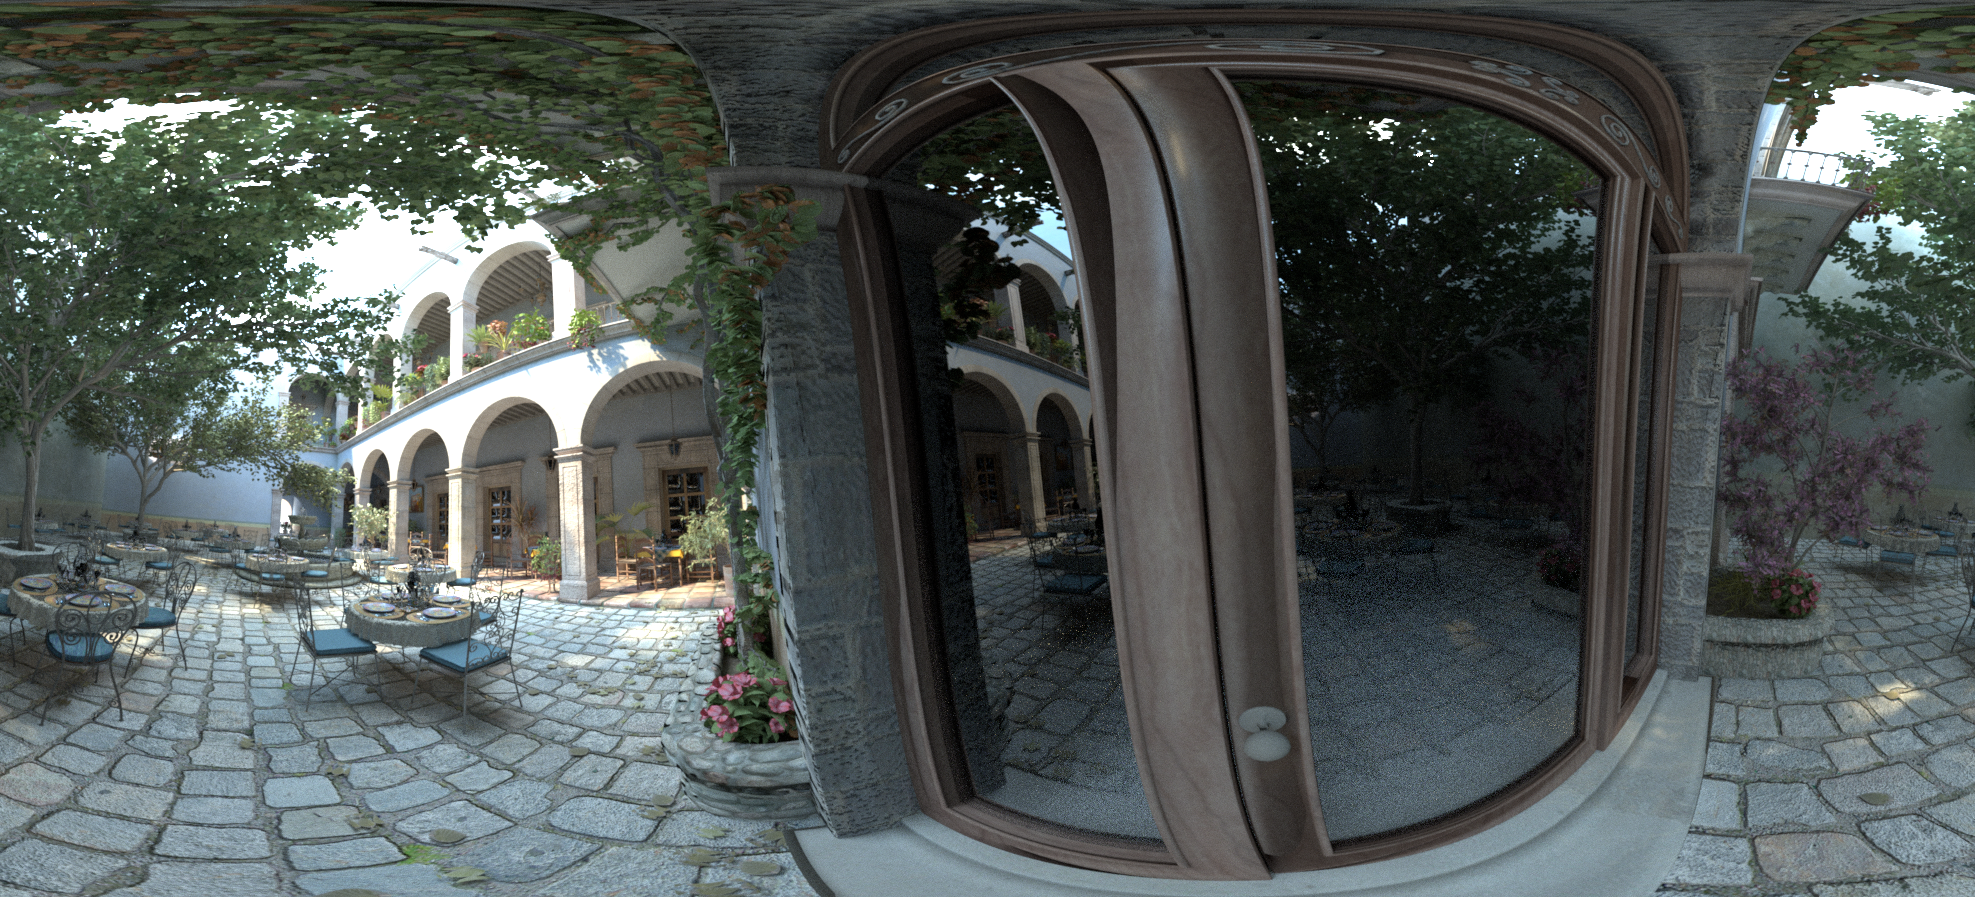
\includegraphics[width=\linewidth]{chap06/sanmiguel-env.png}
    \caption{用\refvar{EnvironmentCamera}{}渲染的San Miguel模型,
    它从相机位置起追踪所有方向的光线。结果图像给出了到达场景中该点所有光线的表示,
    且可用于第\refchap{光源}和第\refchap{光传输I:表面反射}介绍的基于图像的光照技术。}
    \label{fig:6.14}
\end{figure}

\refvar{EnvironmentCamera}{}直接从类\refvar{Camera}{}而非\refvar{ProjectiveCamera}{}导出。
这是因为环境投影是非线性的,不能表示为单个$4\times4$矩阵。
该相机定义在文件\href{https://github.com/mmp/pbrt-v3/tree/master/src/cameras/environment.h}{\ttfamily cameras/environment.h}
和\href{https://github.com/mmp/pbrt-v3/blob/master/src/cameras/environment.cpp}{\ttfamily cameras/environment.cpp}中。
\begin{lstlisting}
`\initcode{EnvironmentCamera Public Methods}{=}`
`\refvar{EnvironmentCamera}{}`(const `\refvar{AnimatedTransform}{}` &CameraToWorld,
        `\refvar{Float}{}` shutterOpen, `\refvar{Float}{}` shutterClose, `\refvar{Film}{}` *film,
        const `\refvar{Medium}{}` *medium)
    : `\refvar{Camera}{}`(CameraToWorld, shutterOpen, shutterClose, film, medium) {
}
\end{lstlisting}
\begin{lstlisting}
`\initcode{EnvironmentCamera Method Definitions}{=}`
`\refvar{Float}{}` `\refvar{EnvironmentCamera}{}`::`\initvar[EnvironmentCamera::GenerateRay]{\refvar{GenerateRay}{}}{}`(const `\refvar{CameraSample}{}` &sample,
        Ray *ray) const {
    `\refcode{Compute environment camera ray direction}{}`
    *ray = `\refvar{Ray}{}`(`\refvar{Point3f}{}`(0, 0, 0), dir, `\refvar{Infinity}{}`,
               `\refvar{Lerp}{}`(sample.`\refvar[CameraSample::time]{time}{}`, `\refvar{shutterOpen}{}`, `\refvar{shutterClose}{}`));
    ray->`\refvar[Ray::medium]{medium}{}` = `\refvar[Camera::medium]{medium}{}`;
    *ray = `\refvar{CameraToWorld}{}`(*ray);
    return 1;
}
\end{lstlisting}

为给该光线计算坐标$(\theta,\phi)$,从栅格图像样本位置中
计算NDC坐标然后缩放它以覆盖$(\theta,\phi)$范围。
接着,用球坐标公式计算光线方向,最后该方向转换到世界空间
(注意因为在相机空间中$y$方向是“向上”,这里球坐标公式中$y$和$z$坐标
和系统其他地方的用法相比是互换了的)。
\begin{lstlisting}
`\initcode{Compute environment camera ray direction}{=}`
`\refvar{Float}{}` theta = `\refvar{Pi}{}` * sample.`\refvar{pFilm}{}`.y / film->`\refvar{fullResolution}{}`.y;
`\refvar{Float}{}` phi = 2 * `\refvar{Pi}{}` * sample.`\refvar{pFilm}{}`.x / film->`\refvar{fullResolution}{}`.x;
`\refvar{Vector3f}{}` dir(std::sin(theta) * std::cos(phi), std::cos(theta),
             std::sin(theta) * std::sin(phi));
\end{lstlisting}